%%%%%%%%%%%%%%%%%%%%%%%%%%%%%%%%%%%%%
% Modelo criado por Vinícius Barros Rodrigues (viniciusbrbio@gmail.com)
% versão 0.2
% abril 2016
%%%%%%%%%%%%%%%%%%%%%%%%%%%%%%%%%%%%%
\documentclass[12pt]{report}
\usepackage[utf8]{inputenc}
\usepackage[brazilian,brazil]{babel}
\usepackage[a4paper,left=4cm,right=3cm,bottom=2.5cm,top=2.8cm]{geometry}
\usepackage{fancyhdr,setspace,float,graphicx,lscape,array,longtable,colortbl,amsmath,amssymb,booktabs,multirow,hyperref,pdfpages}
\usepackage[Sonny]{fncychap}
\usepackage[backend=bibtex,style=authoryear,sorting=nyt,natbib=true]{biblatex}
\ChNameVar{\Large\fontfamily{rm}}
\ChNumVar{\Huge\fontfamily{rm}}
\ChTitleVar{\Large\fontfamily{rm}}

%%%%%%%%%%%%%%%%%%%%%%%%%% 
% Coloque o nome do seu arquivo bib aqui
\addbibresource{references.bib}
%%%%%%%%%%%%%%%%%%%%%%%%%% 

%%%%%%%%%%%%%%%%%%%%%%%%%% 
% Coloque suas imagens e gráficos na pasta images
\graphicspath{{images/}}
% Fique atento: não coloque o "caminho" das suas imagens no texto
%%%%%%%%%%%%%%%%%%%%%%%%%% 

\begin{document}

%%%%%%%%%%%%%%%%%%%%%%%%%%
% Edite cada um dos seguintes arquivos na pasta "preamble"
%%%%%%%%%%%%%%%%%%%%%%%%%%

\input{preamble/cover}

\input{preamble/approval}

\input{preamble/dedication}

\input{preamble/epigraph}

\input{preamble/acknowledgements}

%%%%%%%%%%%%%%%%%%%%%%%%%% SUMÁRIO %%%%%%%%%%%%%%%%%%%
\tableofcontents
\listoffigures
\addcontentsline{toc}{section}{\listfigurename}
\listoftables
\addcontentsline{toc}{section}{\listtablename}
%%%%%%%%%%%%%%%%%%%%%%%%%%%%%%%%%%%%%%%%%%%%%%%%%%%%%%

\input{preamble/abstract}

%%%%%%%%%%%%%%%%%%%%%%%%%%
% Edite cada um dos seguintes arquivos na pasta "chapters"
% Apenas comente ou descomente de acordo com o que precisar
%%%%%%%%%%%%%%%%%%%%%%%%%%

\chapter{Introdução}
\clearpage
\pagenumbering{arabic}
\setcounter{page}{1}
\pagestyle{fancy}
\fancyhead{}
\fancyhead[RO,LE]{Título da tese (opcional)} %%%% preencher (opcional)
\fancyfoot{}
\fancyfoot[LE,RO]{\thepage}
\fancyfoot[LO,CE]{Capítulo \thechapter}
\fancyfoot[CO,RE]{Autor (opcional)} %%%% preencher com nome (opcional)
%%%%%%%%%%%%%%%%% COLE SEU TEXTO AQUI: %%%%%%%%%%%%%%%%%%%%%%%
\chapter{\sc Um título}
\lipsum[2-2] \citep{lamport1986latex} 
\begin{figure}[h]
\centering
\caption{Minha figura}
 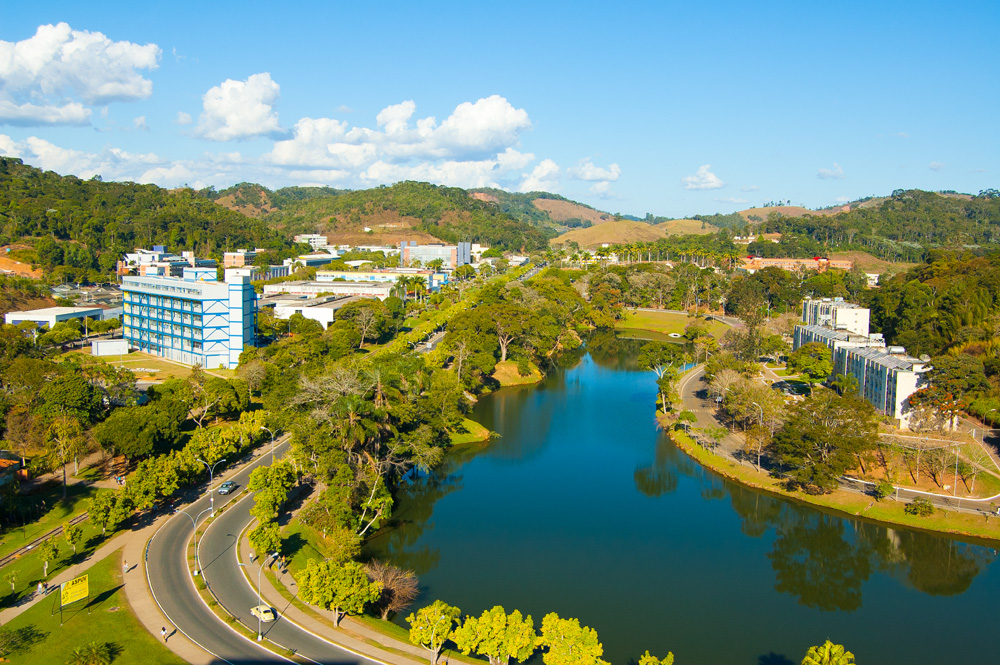
\includegraphics[scale=0.2]{ufv.jpg}
\end{figure}
\section{Seção nova}
\lipsum[2-3]
%%%% APAGAR O EXEMPLO ACIMA








%
\chapter{Título do cap dois}
\input{chapters/chapter02}
%
% \chapter{Capítulo três título}
% \input{chapters/chapter03}
%
% \chapter{Capítulo quatro título}
% \input{chapters/chapter04}
%
% \chapter{Conclusão}
% \input{chapters/conclusion}
%
% \appendix
% \chapter{Apêndice}
% \input{chapters/appendix}


%%%%%%%%%%%%%%%%%%%%%%%%%%% ADICIONANDO ANÁLISES ESTATÍSTICAS EM PDF %%%%%%%%%%%%%%%%%
% Descomente e coloque o nome do seu arquivo
%\includepdf[pages=-]{myfile.pdf}
%%%%%%%%%%%%%%%%
  
\end{document}
